  % Background: Syntax, type systems, and operational semantics

  In the formal study of a programming langugage, one may define a language
  in three parts: syntax, type system, and operational semantics.
  \begin{itemize}
    \item The {\em syntax} is written in the form of a (usually)
      context-free grammar describing the allowable expressions.
    \item A {\em type system} further refines the set of allowable
      expressions into a set of {\em meaningful} expressions, and provides
      a mapping between an expression and an approximation of its meaning.
      Type systems are usually designed in conjunction with the operational
      semantics to have the property that {\em well-typed programs don't go
      wrong}, i.e., every expression assigned a meaning by the type system
      should have a well-defined runtime behavior.
    \item An {\em operational semantics} defines how runnable programs
      (e.g. a function applied to an argument) {\em reduce} to values. This
      part of the definition describes how actual computation takes place
      when programs in the language are run. It is important to note that
      the operational semantics need not reflect the actual {\em
      implementation} of the language, nor is it specific to a ``compiled''
      versus ``interpreted'' understanding of the language: it is simply a
      mathematical specification for how any compiler or interpreter for
      the language should behave.
  \end{itemize}
  
  Providing a formal language definition in programming languages research
  has several purposes. One is that it enables researchers to explore
  and prove formal properties of their language, such as {\em well-typed
  programs don't go wrong}, or in a language for concurrency, a property
  like deadlock freedom. However, an even more crucial advantage of a
  language specification is not mathematical rigor but human capacity to do
  science. A language definition is a {\em specification}, similar to an
  application programmer interface (API) or an IEEE standard: it describes
  an unambiguous interface to the language along an {\em abstraction
  boundary} that other human beings may access, understand, and implement,
  without knowing the internals of a language implementation.  It is a
  necessary component of reproducibility of research, and it allows
  researchers to build on each other's work. We believe that an embrace of
  the formal specification in games research can play a similarly important
  function.

  Having provided loose definitions of these terms, we now wish to draw out
  the analogy between a {\em language} specification and a {\em game}
  specification. To treat a game in this manner, we wish to consider player
  affordances and actions, as well as their behavior (mechanics) in the
  context of the game's running environment. We summarize the components of
  this correspondence in Table~\ref{tab:correspondence}.

  \begin{table}
  \begin{tabular}{ll}
    PL concept & Game concept\\
    \hline
    Syntax & Recognized player actions \\
    Type system & Meaningful player actions \\
    Operational semantics & Game mechanics \\
    Runtime store & Game world \\
    Normalized programs & Play traces 
  \end{tabular}
  \label{tab:correspondence}
  \end{table}

  \newcommand{\cmove}{\mathsf{move}}
  \newcommand{\ctake}{\mathsf{take}}

  We will use as a running example a minimal virtual environment with two
  player actions: (1) movement through a discrete set of rooms in a
  pre-defined map ($\cmove$); (2) acquiring objects placed in those rooms to store in
  a player inventory ($\ctake$).  We can consider several possibilities in
  the design space of interfaces for such a game:

  \begin{itemize}
   \item {\bf Point-and-Click:} A first-person viewpoint interface where the
     meaning of each click is defined based on the region the cursor falls
     in. Clicking near any of the four screen edges moves in that
     direction; clicking on a sprite representing an item takes it.
  \item {\bf Bird's-Eye:} A top-down viewpoint interface where the player can see multiple
    rooms at once, and can click on rooms and objects that are far away,
    but those clicks only do something to objects in the same room or
    adjacent rooms.
  \item {\bf WASD+:} A keyboard or controller-based interface with
    directional buttons (e.g. arrow keys or WASD) move an avatar in the
    correspondingi direction, and a separate key or button expresses
    the $\ctake$ action, which takes any object in the same room. (This
    interface may be used for either of the two views described above.)
  \item{\bf Command-Line:} The player interacts by typing free-form text, 
    which is then parsed into commands, such as \verb|take lamp| and \verb|move north|.
  \item{\bf Hypertext}: A choice-based interface where all available options are
    enumerated as textual links from which the player chooses.
  \end{itemize}

  \begin{figure*}
    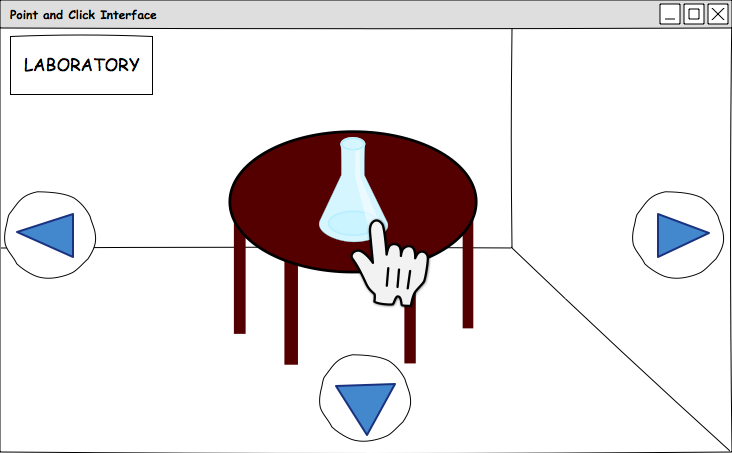
\includegraphics[width=0.4\textwidth]{../uis/point-and-click.png}
    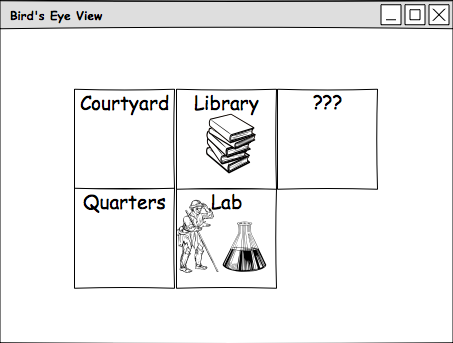
\includegraphics[width=0.4\textwidth]{../uis/birds-eye-view.png}

    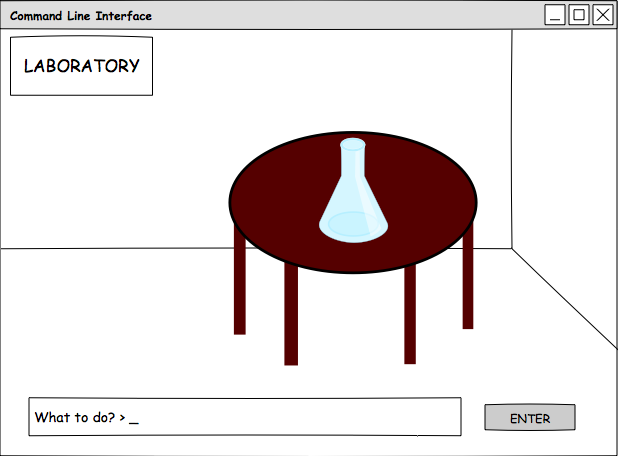
\includegraphics[width=0.4\textwidth]{../uis/parser.png}
    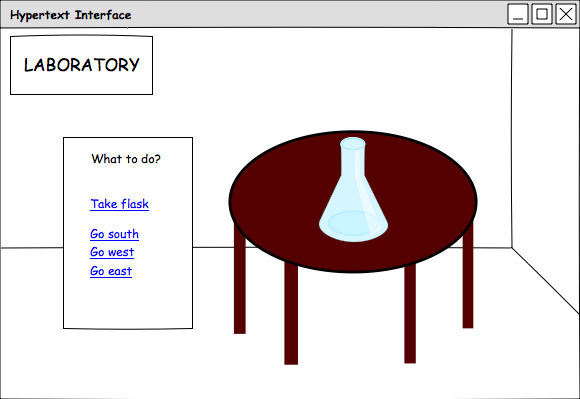
\includegraphics[width=0.4\textwidth]{../uis/hypertext.png}
  \end{figure*}

  These interfaces are shown in Figure(XXX) (with the exception of WASD+,
  which is visually indistinguishable from Bird's Eye).
  In the following subsections, we will consider these possibilities in
  light of design choices relevant to the specified aspect of PL design.

  \subsection{Player actions as syntax}

  The {\em syntax} of a game is its space of recognized player intentions.
  Note that {\em intention} is different from {\em action} in the sense
  that we don't necessarily expect each well-formed intention to change
  anything about the game state: a player can intend to move north, but if
  there is no room to the north of the player when she expresses this
  intent, no change to the game's internal state will occur. Nonetheless,
  depending on the design goals of the game, we may wish to recognize this
  as a valid intent so that the game may respond in some useful way (e.g.
  with feedback that the player cannot move in that direction).
  
  In our example game, the choice of syntax answers questions such as: can
  the player click anywhere, or only in regions that have meaning? Can the
  player type arbitrary commands, or should we provide a menu or
  auto-complete text so as to prevent the player from entering meaningless
  commands?
  In PL, we can formalize these decisions by describing an {\em abstract
  syntax} for our language, which is typically assumed to be context-free
  and thus specified as a Bachus-Naur Form (BNF) grammar. As one example,
  the BNF for the keyboard-based interface might look like:

  \begin{eqnarray*}
  direction &::=& \mathsf{north} \mid \mathsf{south} \mid \mathsf{east}
    \mid \mathsf{west} \\
  intent &::=& \cmove\  \langle direction \rangle \mid \ctake
  \end{eqnarray*}

  XXX more here...

  BNF for interface 2:\\
  \verb/go <dir> | take <thing>/\\
  n.b. larger set of allowable utterances; meaning is less contextual
  (easier to infer by itself what parts of the game state it will depend
  on)

  BNF for interface 3:\\
  \verb/move <dir>/\\
  n.b. much {\em more} contextual; it's impossible to infer what each
  action will ``do'' in the game and which parts of the game environment it
  depends on

  Additive vs. subtractive affordances:

  Just like with the rest of a game's rules, its language of play has both
  additive and subtractive properties: it provides the menu of options for
  what types of things are {\em permissible}, i.e. likely to result in
  meaningful interaction with the game system, but it also establishes
  which utterances are {\em disallowed}, i.e. that it is not meaningful to
  say ``take'' without providing an object to the command.

  ... is the grammar for a blank text field that or is it just any typed
  string, and the type system what enforces the grammatical structure?
  (XXX)

  \subsection{Structured affordances as type systems}
  
  Whether an utterance is {\em meaningful} or not will depend on
  the runtime game state, and is a distinct question from whether it is
  well-formed. For example, whether or not we can {\em take
  flask} depends on whether the flask is present, or indeed whether a {\em
  flask} is even a recognized game object. But unless ill-formed intents can be
  recognized a priori (such as: if we know the complete set of possible
  game objects ahead of time and can reject commands that refer to entities
  outside of that set), we must treat this command as well-formed {\em
  syntax} and relegate its failure to integrate with the runtime game
  environment to the {\em mechanics} (operational semantics).

  However, we can rule out an approximation of ill-formed utterances using
  type systems. For example, if we know the ...
  (only take portable things, only talk to characters, etc - could be
  specified at the grammar level)
  
  Providing the player with {\em only the option of saying} those
  utterances that ``make sense'' in this regard corresponds to a strong
  static type system: e.g. choice-based interface to parser-based
  commands...

  Consider fishing minigame in Stardew Valley: the player only has a way of
  {\em expressing} a ``reel in fishing line'' verb in the context of the
  fishing minigame. This action has no corresponding utterance in the main
  interface of the game.

  XXX analogy to structure editors, visual prog environments, discoverable
  choice-based interfaces...


  \subsection{Game environment as external runtime}

  To characterize mechanics, we will also need an account of expressions
  permissible in the game's language (e.g. display a room, make a sound,
  make an object disappear, etc. --- things more commonly accounted for in
  formal game description languages). 

  We will also need to characterize ``hidden'' state of the game...
  predicate syntax... locations of things, adjacency graph to describe the
  world map

  World state $\sigma$; game expressions $e_g$; used in the judgments
  defining operational semantics below


  \subsection{Mechanics as operational semantics}

  XXX - need to explain step syntax, as well as inference rules

  \newcommand{\Player}[4]{\ensuremath{#1{:}\left< {#2} , {#3} , {#4} \right>}}
\newcommand{\PropIsTrue}[2]{\ensuremath{#1 \vdash #2~\textsf{true}}}
\newcommand{\StepsTo}[4]{\ensuremath{\left< #1 ; #2 \right> \longrightarrow \left< #3 ; #4 \right>}}

\section{Precise player-game dynamics via operational semantics}
\label{sec:opsem}

The player consists of a 

The operational semantics employs notions of the game and player states.

The following BNF definitions give meta variable conventions (the left-hand-side variable names) and syntactic cases (the right-hand-side of each rule).


\begin{figure*}
\small

\begin{tabular}{l|l}

\begin{minipage}{0.7\textwidth}
\begin{tabular}{lccll}
propositions   & $P$ & $::=$ & $\cdots$ & Game world propositions~(See~$\PropIsTrue{G}{P}$)
\\
player command & $C$ & $::=$ & $\cdot$ $~|~$ $c$ & Unit and atomic commands (0 and 1 turns, resp.)
\\
               &     & $~|~$ & $C_1~{;}~C_2$ & Command sequences (multi-turn commands)
\\
               &     & $~|~$ & $\textsf{until}~P~\textsf{do}~C$ & Command loops (e.g., for player skills)
\\
atomic command & $c$ & $::=$ & $\textsf{grasp}~i$ & Attempt to place~object$i$ into player's hand
\\
               &     & $|$   & $\textsf{drop}$ & Drop the held object, if any
\\
               &     & $|$   & $\textsf{giveTo}~i$ & Give held object to another~(named~$i$)
\\
               &     & $|$   & $\textsf{takeFrom}~i$ & Take hold of object from another~(named~$i$)
\\
               &     & $|$   & $\textsf{moveTo}~i$ & Move adjacent to object, place or agent~(named~$i$)
\\
               &     & $|$   & $\textsf{moveThrough}~i$ & Move through opening~(named~$i$)
\\[5mm]
unique IDs & $i,j$ & $::=$ & $\cdots$ & (\emph{abstract}, e.g., numbers, symbols, noun phrases)
\\
game state & $G$ & $::=$ & $\cdots$ & (\emph{abstract})
\\
player state & $p$ & $::=$ & $$ & Player identity, bag~$B$, hand~$h$ and commands~$C$
\\
unit space (hand) & $s,h$ & $::=$ & $\square~|~i$ & An empty space, or an object~(named~$i$)
\\
aggregate space (bag) & $S,B$ & $::=$ & $\cdot~|~s::S$ & Zero or more unit spaces
\end{tabular}
\end{minipage}

&

\begin{minipage}{0.3\textwidth}
\[
\begin{array}{ll}
\fbox{$G_1 \equiv G_2$}~\textrm{World equivalence}
\\
\fbox{$b_1 \equiv b_2$}~\textrm{Bag equivalence}
\\
\fbox{$\PropIsTrue{G}{P}$} 
\\
\textrm{In world~$G$, proposition~$P$ is true}.
\\[2mm]
\fbox{$\StepsTo{G}{p}{G'}{p'}$}
\\[2mm]

\infer
{  
\StepsTo
{G}{\Player{i}{B_1}{\square} {\textsf{grasp}~$j$}}
{G}{\Player{i}{B_2}{j}{\cdot}}
}
{
B_1 \equiv j :: B_2
}


\end{array}
\]
\end{minipage}


\end{tabular}

\caption{Definitions for an operational semantics: Captures precise
  player-game dynamics for a primitive adventure game.}
\end{figure*}

  
  \newcommand{\stepsto}{\rightsquigarrow}

  Judgment: $\sigma; e_p \stepsto \sigma'; e_g$ \\
  where $e_p$ is a player expression and $e_g$ is a game expression, and
  $\sigma$ and $\sigma'$ are game states. This judgment should be read:
  ``Under state $\sigma$, the game responds to player action $e_p$ by
  changing to state $\sigma'$ and conveying information $e_g$.''

  Mechanics of interface 1:

  \[
    \infer{
      \sigma, at(R); PLAYER: move<dir> \stepsto \sigma, at(R'); GAME:
      display(R')
    }
    {
      indir(dir, R, R') \in \sigma
    }
  \]


  \[
    \infer{
      \sigma, at(R); PLAYER: move<dir> \stepsto 
      \sigma; GAME: \mathsf{fail\_feedback}
    }
    {
      indir(dir, R, R') \notin \sigma
    }
  \]

  XXX more rules

  n.b. this semantics is not really ``complete'' in the sense that it does
  not define meaning for sequences of actions, just single exchanges... how
  to compose actions?

  \subsection{Play traces as (normalized) programs}
  
  Argument for having a syntactically-well-founded structured term for a
  play trace

  \subsection{Theorems?}

  While it is not often considered of high priority for game designers to
  prove theorems about their software, and in fact a rich culture is
  enjoyed around the concept of {\em glitches} in games programs, a
  meticulous designer may still wish to understand the scope, complexity,
  and compatibility of her game approximated by compatibility between 
  player affordances and game rules. A formal examination of the game's
  properties, when studied as a programming language, can provide just
  that:

  Well-typed programs don't go wrong ~= every possible player utterance has
  a defined meaning within the game rules

  XXX example of this failing?

